\documentclass[conference]{IEEEtran}

\ifCLASSINFOpdf
\usepackage[pdftex]{graphicx}
\usepackage{float}

\hyphenation{op-tical net-works semi- -tor}

\begin{document}
\title{Intermediate report: Synthesis of sound with nodes}

\maketitle

\begin{abstract}
This report provides an intermediate overview of an ongoing project focused on visual sound synthesis using nodes. The project aims to develop an intuitive and interactive tool that allows users to generate and manipulate sound waves visually, bypassing the need for traditional programming approaches. Each node in the system serves a specific purpose: sound generation, manipulation, or output to an audio device. This report discusses the project’s goals, reviews related work in the field, describes progress made in application development, and outlines future directions for the project.
\end{abstract}

\IEEEpeerreviewmaketitle

\section{Goals}
The primary objective of this project is to design and implement a tool for computer sound synthesis based on a node-based interface. The tool seeks to simplify the process of learning and experimenting with sound synthesis by eliminating the need for coding skills. 
The key node categories, which provide the following features, are:\label{basicsaudionodes}
\begin{itemize}
    \item sound generation Nodes: nodes capable of producing audio signals, such as sine wave generators or file input nodes;
    \item sound manipulation Nodes: tools for modifying audio signals, such as adders, multipliers, pass-through nodes, and various filters;
    \item components for directing audio to outputs, such as speakers, file writers, or other audio devices.
\end{itemize}
Users will be able to arrange nodes on a virtual canvas and connect them with wires, creating pathways for data flow between nodes.  The application emphasizes usability and interactivity to improve the learning process and enable creativity in sound synthesis without requiring programming expertise.

\section{Related work}
A similar project is a project \textit{AudioNodes}~\cite{audionodes}, which is used to create sounds, add effects, and compose original creations with a modular interface. This project aims to design and implement a similar tool, where users will be able to arrange and connect nodes to synthesize sound. An example graph, made with \textit{AudioNodes}, is shown in figure~\ref{fig:audionodes}.

\textit{AudioNodes} is a digital audio workstation based on interconnectable modules, called nodes. Each AudioNode can:
\begin{itemize}
    \item produce audio on its own and output it through its output port;
    \item take audio input and manipulate it (change gain or add reverb) and then output the modified audio;
    \item nodes that output the audio to the system or to an audio file when exporting.
\end{itemize}
The nodes in \textit{AudioNodes} are connected with \textit{audio connections} (blue) carrying a sampled audio signal \cite{audionodes}. More information about the tool can be found on the tool's documentation page~\cite{audionodesdocs}

\begin{figure}[H]
\centering
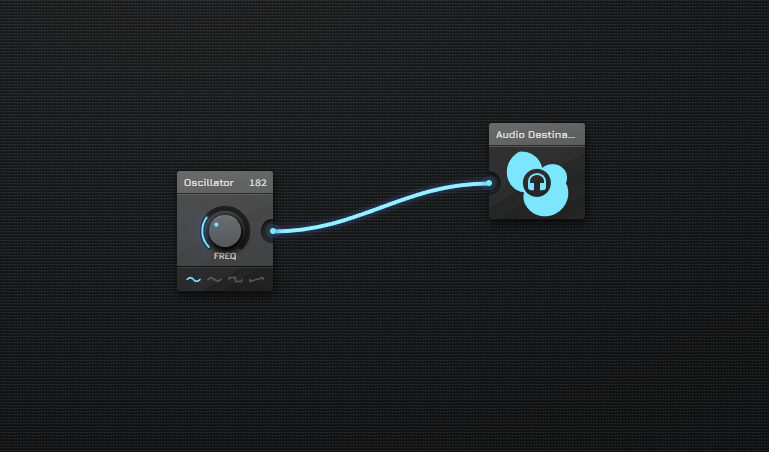
\includegraphics[width=1.0\linewidth]{graphics/audionodes.png}
\caption{Example graph, made with the tool \textit{AudioNodes}~\cite{audionodes}. The graph generates a sine wave and outputs it to the default audio output device.}
\label{fig:audionodes}
\end{figure}

\section{Progress}
The development process began by setting up the project environment for building and managing dependencies. I chose the \textit{CMake} build system~\cite{cmake}, a tool for managing and configuring C++ projects.
To implement the graphical user interface (GUI), several external libraries were integrated into the project:
\begin{itemize}
    \item \textit{OpenGL}~\cite{opengl} for rendering the GUI. \textit{Glad}~\cite{glad} was utilized to provide the necessary bindings for \textit{OpenGL};
    \item \textit{GLFW}~\cite{glfw} for creating windows and receiving input and events;
    \item \textit{ImGui}~\cite{imgui} and an \textit{ImGui} extension \textit{Imgui-Node-Editor}~\cite{imguinodeeditor} for GUI implementation for the node-based graph editor;
    \item \textit{RtAudio}~\cite{rtaudio} for handling audio input and output, providing the necessary functionality to stream and manipulate sound in real time.
\end{itemize}
All dependencies were chosen to keep the application cross-platform and as lightweight as possible. Each dependency was installed and included in the project, and the functionalities were tested to make sure they work correctly.

After that, the project was organized into logical independent components, which will be developed independently. The codebase was separated into two parts:
\begin{itemize}
    \item \texttt{AudioEditor} for editing and constructing graphs;
    \item \texttt{AudioEngine} for implementing nodes and generating, playing, and manipulating sound.
\end{itemize}
First, groundwork for the \texttt{AudioEditor} was implemented, where we created an empty window and initialized and rendered to it with \textit{ImGui}~\cite{imgui}. Then, the \textit{Imgui-Node-Editor}~\cite{imguinodeeditor} library was initialized on that window, and an empty workspace was implemented, where the graph would be constructed. A simple node was drawn on the workspace to test \textit{Imgui-Node-Editor}~\cite{imguinodeeditor}. We also prepared the necessary callbacks for handling input and errors. The current window state is shown in figure~\ref{fig:editor-window}.

\begin{figure}[H]
\centering
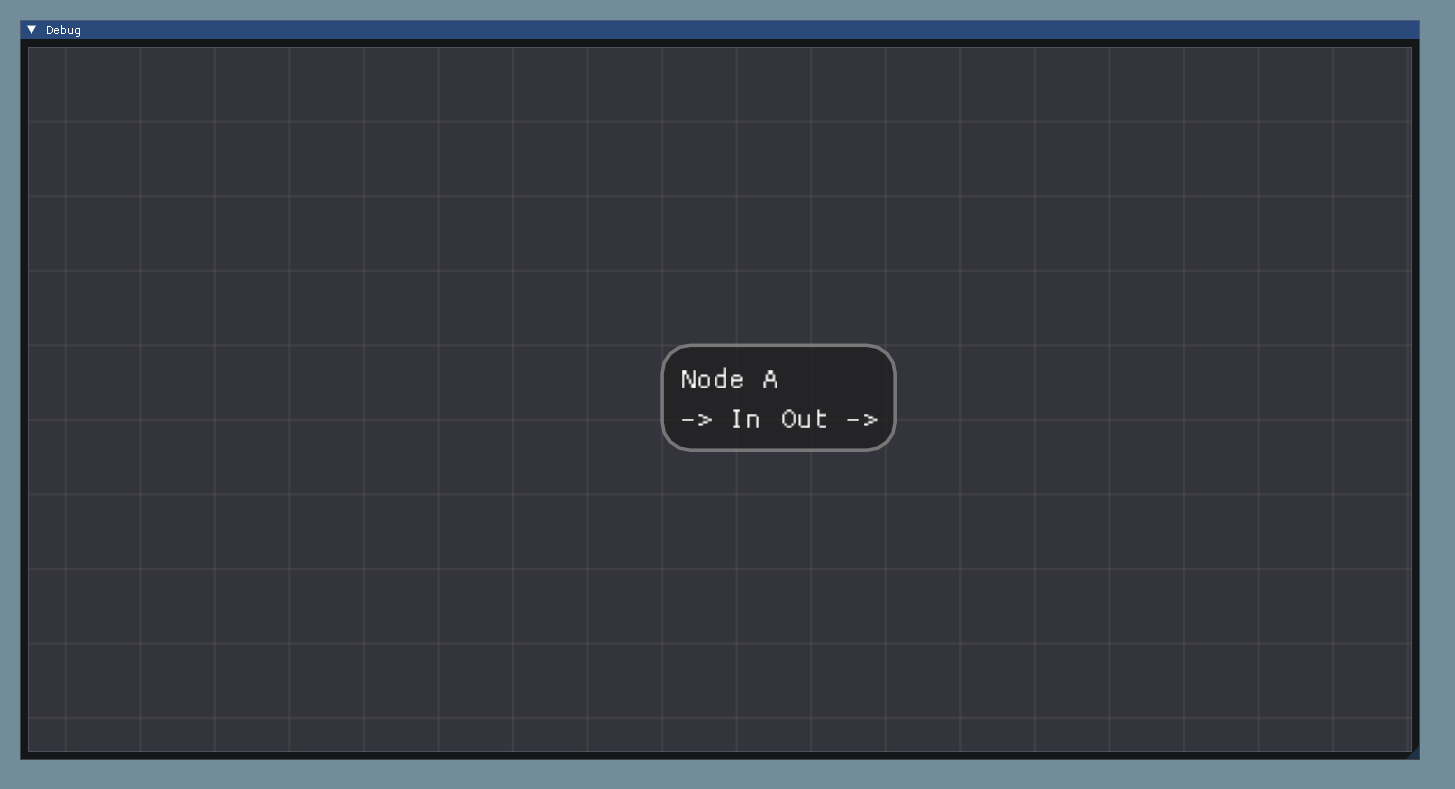
\includegraphics[width=1.0\linewidth]{graphics/editor-window.png}
\caption{Workspace for graph construction, implemented in \textit{Imgui-Node-Editor}~\cite{imguinodeeditor} with a simple example node drawn.}
\label{fig:editor-window}
\end{figure}

Then, we started designing and implementing the application programming interface (API) for \textit{AudioNodes}. We defined the following classes:
\begin{itemize}
    \item \textit{AudioPin} for defining inputs and outputs;
    \item \textit{AudioLink} for linking \textit{AudioPins} together;
    \item \textit{AudioNode} for sound generation, manipulation, and streaming.
\end{itemize}

After that, we began implementing the first two nodes:
\begin{itemize}
    \item \textit{SineOscillatorNode} for generating a sine wave;
    \item \textit{LineOutNode} for outputting audio to the default device.
\end{itemize}

Finally, we tested its functionality by linking the two nodes together in code and producing a simple sound, shown in figure~\ref{fig:sine-oscillator-demo}

\begin{figure}[H]
\centering
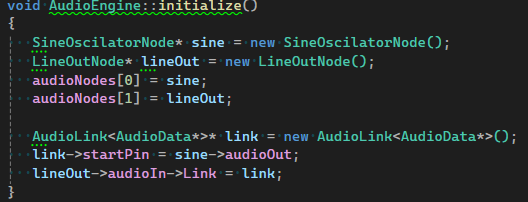
\includegraphics[width=1.0\linewidth]{graphics/sine-oscilator-demo.png}
\caption{Code used to test the API for the \textit{AudioEngine} part of the application. It creates two \textit{AudioNodes} and connects them with an \textit{AudioLink} to generate a simple sound.}
\label{fig:sine-oscillator-demo}
\end{figure}

\section{Future work}
The future work on this project will involve improving the \textit{AudioEngine} API and making it easier to define new \textit{AudioNodes} for different purposes. The \textit{AudioEditor} will need to be implemented to support the construction and editing of the graph, and finally, more nodes will be implemented for more advanced sound generation and manipulation.

\begin{thebibliography}{1}
\bibitem{audionodes}
Audio Nodes https://www.audionodes.com/

\bibitem{audionodesdocs}
Audio Nodes https://www.audionodes.com/docs/

\bibitem{cmake}
CMake https://cmake.org/

\bibitem{opengl}
OpenGL https://www.opengl.org/

\bibitem{glad}
Glad https://github.com/Dav1dde/glad

\bibitem{glfw}
GLFW https://www.glfw.org/

\bibitem{imgui}
ImGui:~API for GUI in C++ https://github.com/ocornut/imgui

\bibitem{imguinodeeditor}
Imgui Node Editor:~Implementation of a node editor using ImGui https://github.com/thedmd/imgui-node-editor

\bibitem{rtaudio}
RtAudio:~API for realtime audio input/output in C++ https://www.music.mcgill.ca/~gary/rtaudio/

\end{thebibliography}

\end{document}
